% Change the following title and label as desired.
\section{Design and Implementation}
\label{sec:designandimplementation}

\subsection{System Description}
\label{sec:systemdescription}
The research and system development are applied according to the design and implementation described in this chapter. This system design includes the concept of creation, design, flow, and infrastructure implementation depicted in a Block Diagram. The design and implementation are illustrated using figures and will be explained from data collection in the form of images, analysis of the model created to detect human objects, and the system using the model as shown in Figure \ref{fig:System Block Diagram} and detailed in each sub-section.

\begin{figure}[H]
  \centering

  % Change with the desired image file name and size
  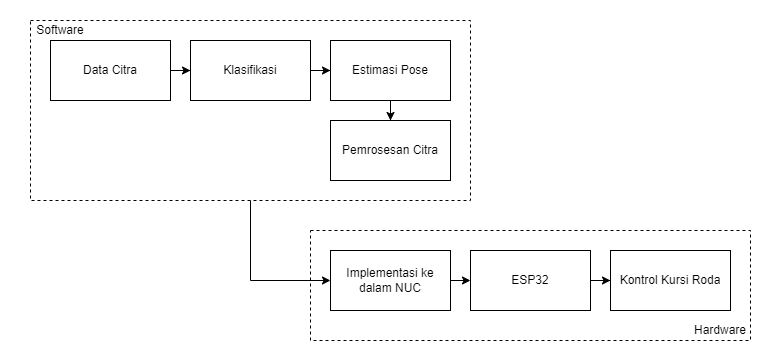
\includegraphics[scale=0.3]{gambar/Agungbaru blok.drawio.png}

  % Change with the desired image caption
  \caption{System Block Diagram}
  \label{fig:System Block Diagram}
\end{figure}

\subsection{Hardware}
Hardware design is conducted according to the flow described in this subsection. This design will be presented with a flow block diagram that represents the flow of this hardware design. Figure \ref{fig:Hardware Block Diagram} shows the hardware block diagram as follows:
\begin{figure}[H]
  \centering

  % Change with the desired image file name and size
  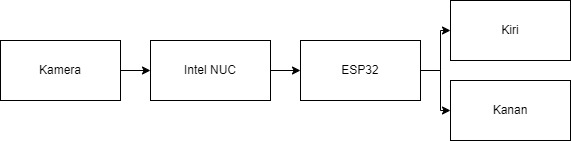
\includegraphics[scale=0.3]{gambar/hardware.jpg}

  % Change with the desired image caption
  \caption{Hardware Block Diagram}
  \label{fig:Hardware Block Diagram}
\end{figure}

\subsection{Software}
Software design is conducted according to the flow described in this subsection. This design will be presented with a flow block diagram that represents the flow of this software design. Figure \ref{fig:Software Block Diagram} shows the software block diagram as follows:

\begin{figure}[H]
    \centering
    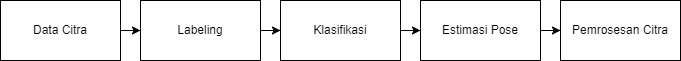
\includegraphics[scale = 0.3]{gambar/labeling.jpg}
    \caption{Software Block Diagram}
    \label{fig:Software Block Diagram}
\end{figure}

\subsection{YoloV8 Classification}
In the classification process, each image that has undergone the labeling process will be recognized using YoloV8, which has been trained to recognize humans in the images. The model will provide output according to the human class, and the classification results will be used as a reference for position in the detection grid.

The model used has an output class of Human, and the values provided by the model include the \emph{Bounding Box} and Confidence Score. The process flow can be seen in Figure \ref{fig:YoloV8 Architecture Visualization}, which is an architectural block diagram.
\begin{figure}[H]
  \centering
  % Change with the desired image file name and size
  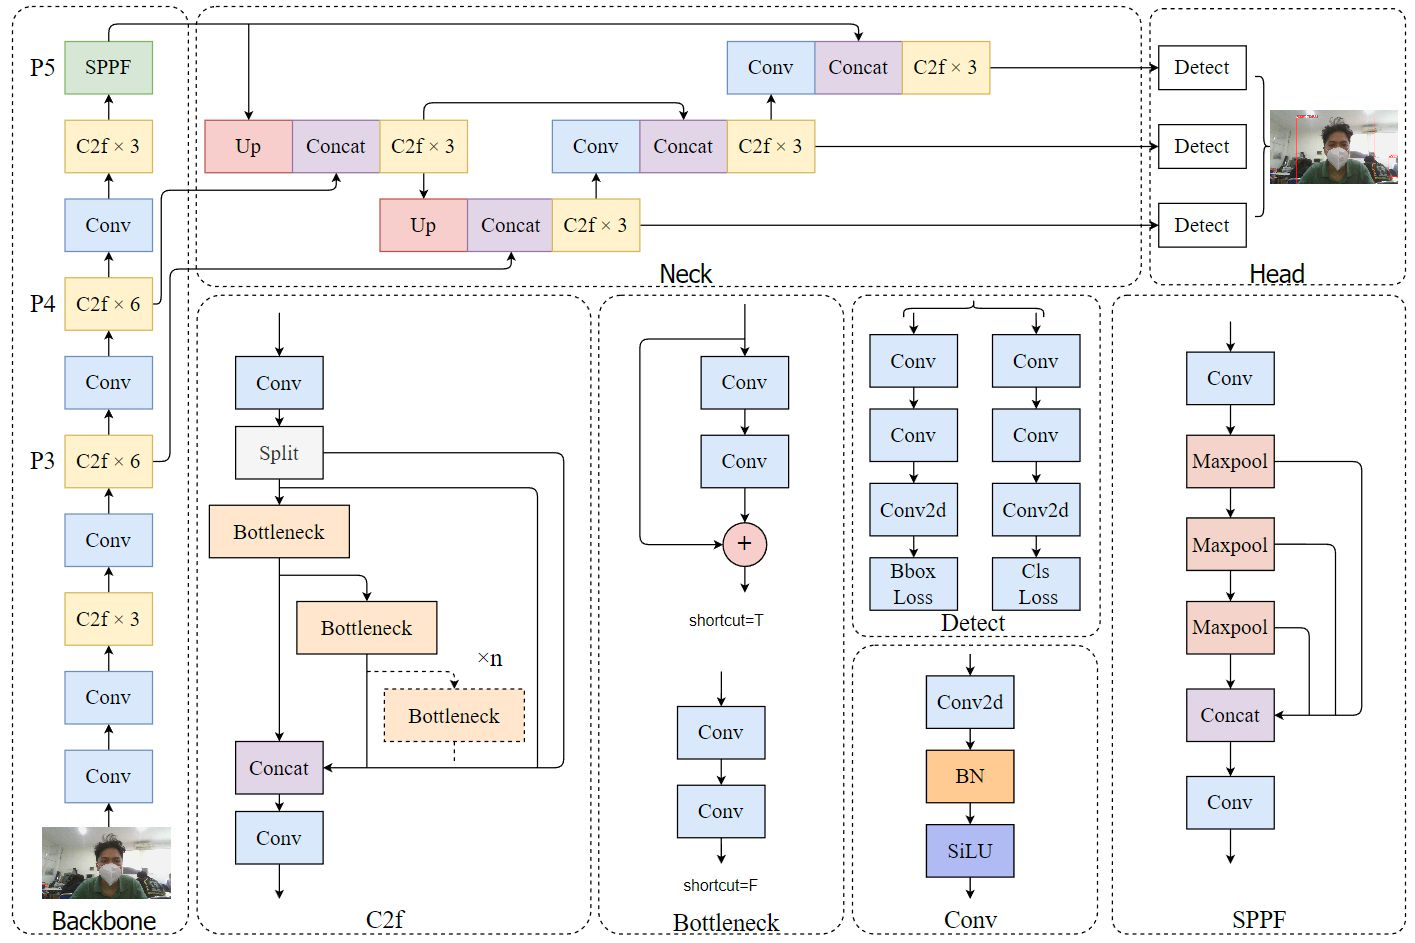
\includegraphics[scale=0.19]{gambar/bab3_arsagung.png}
  % Change with the desired image caption
  \caption{YoloV8 Architecture Visualization}
  \label{fig:YoloV8 Architecture Visualization}
\end{figure}

In Figure \ref{fig:YoloV8 Architecture Visualization with VisualKeras}, blue indicates convolutional layers present in the backbone, neck, and head. Yellow indicates C2f residual blocks with convolution. Light green indicates SPPF layers for Spatial Pyramid Pooling Fast. Pink indicates UpSampling layers. Purple indicates Concatenate layers for combining feature maps.

\begin{figure}[H]
  \centering
  % Change with the desired image file name and size
  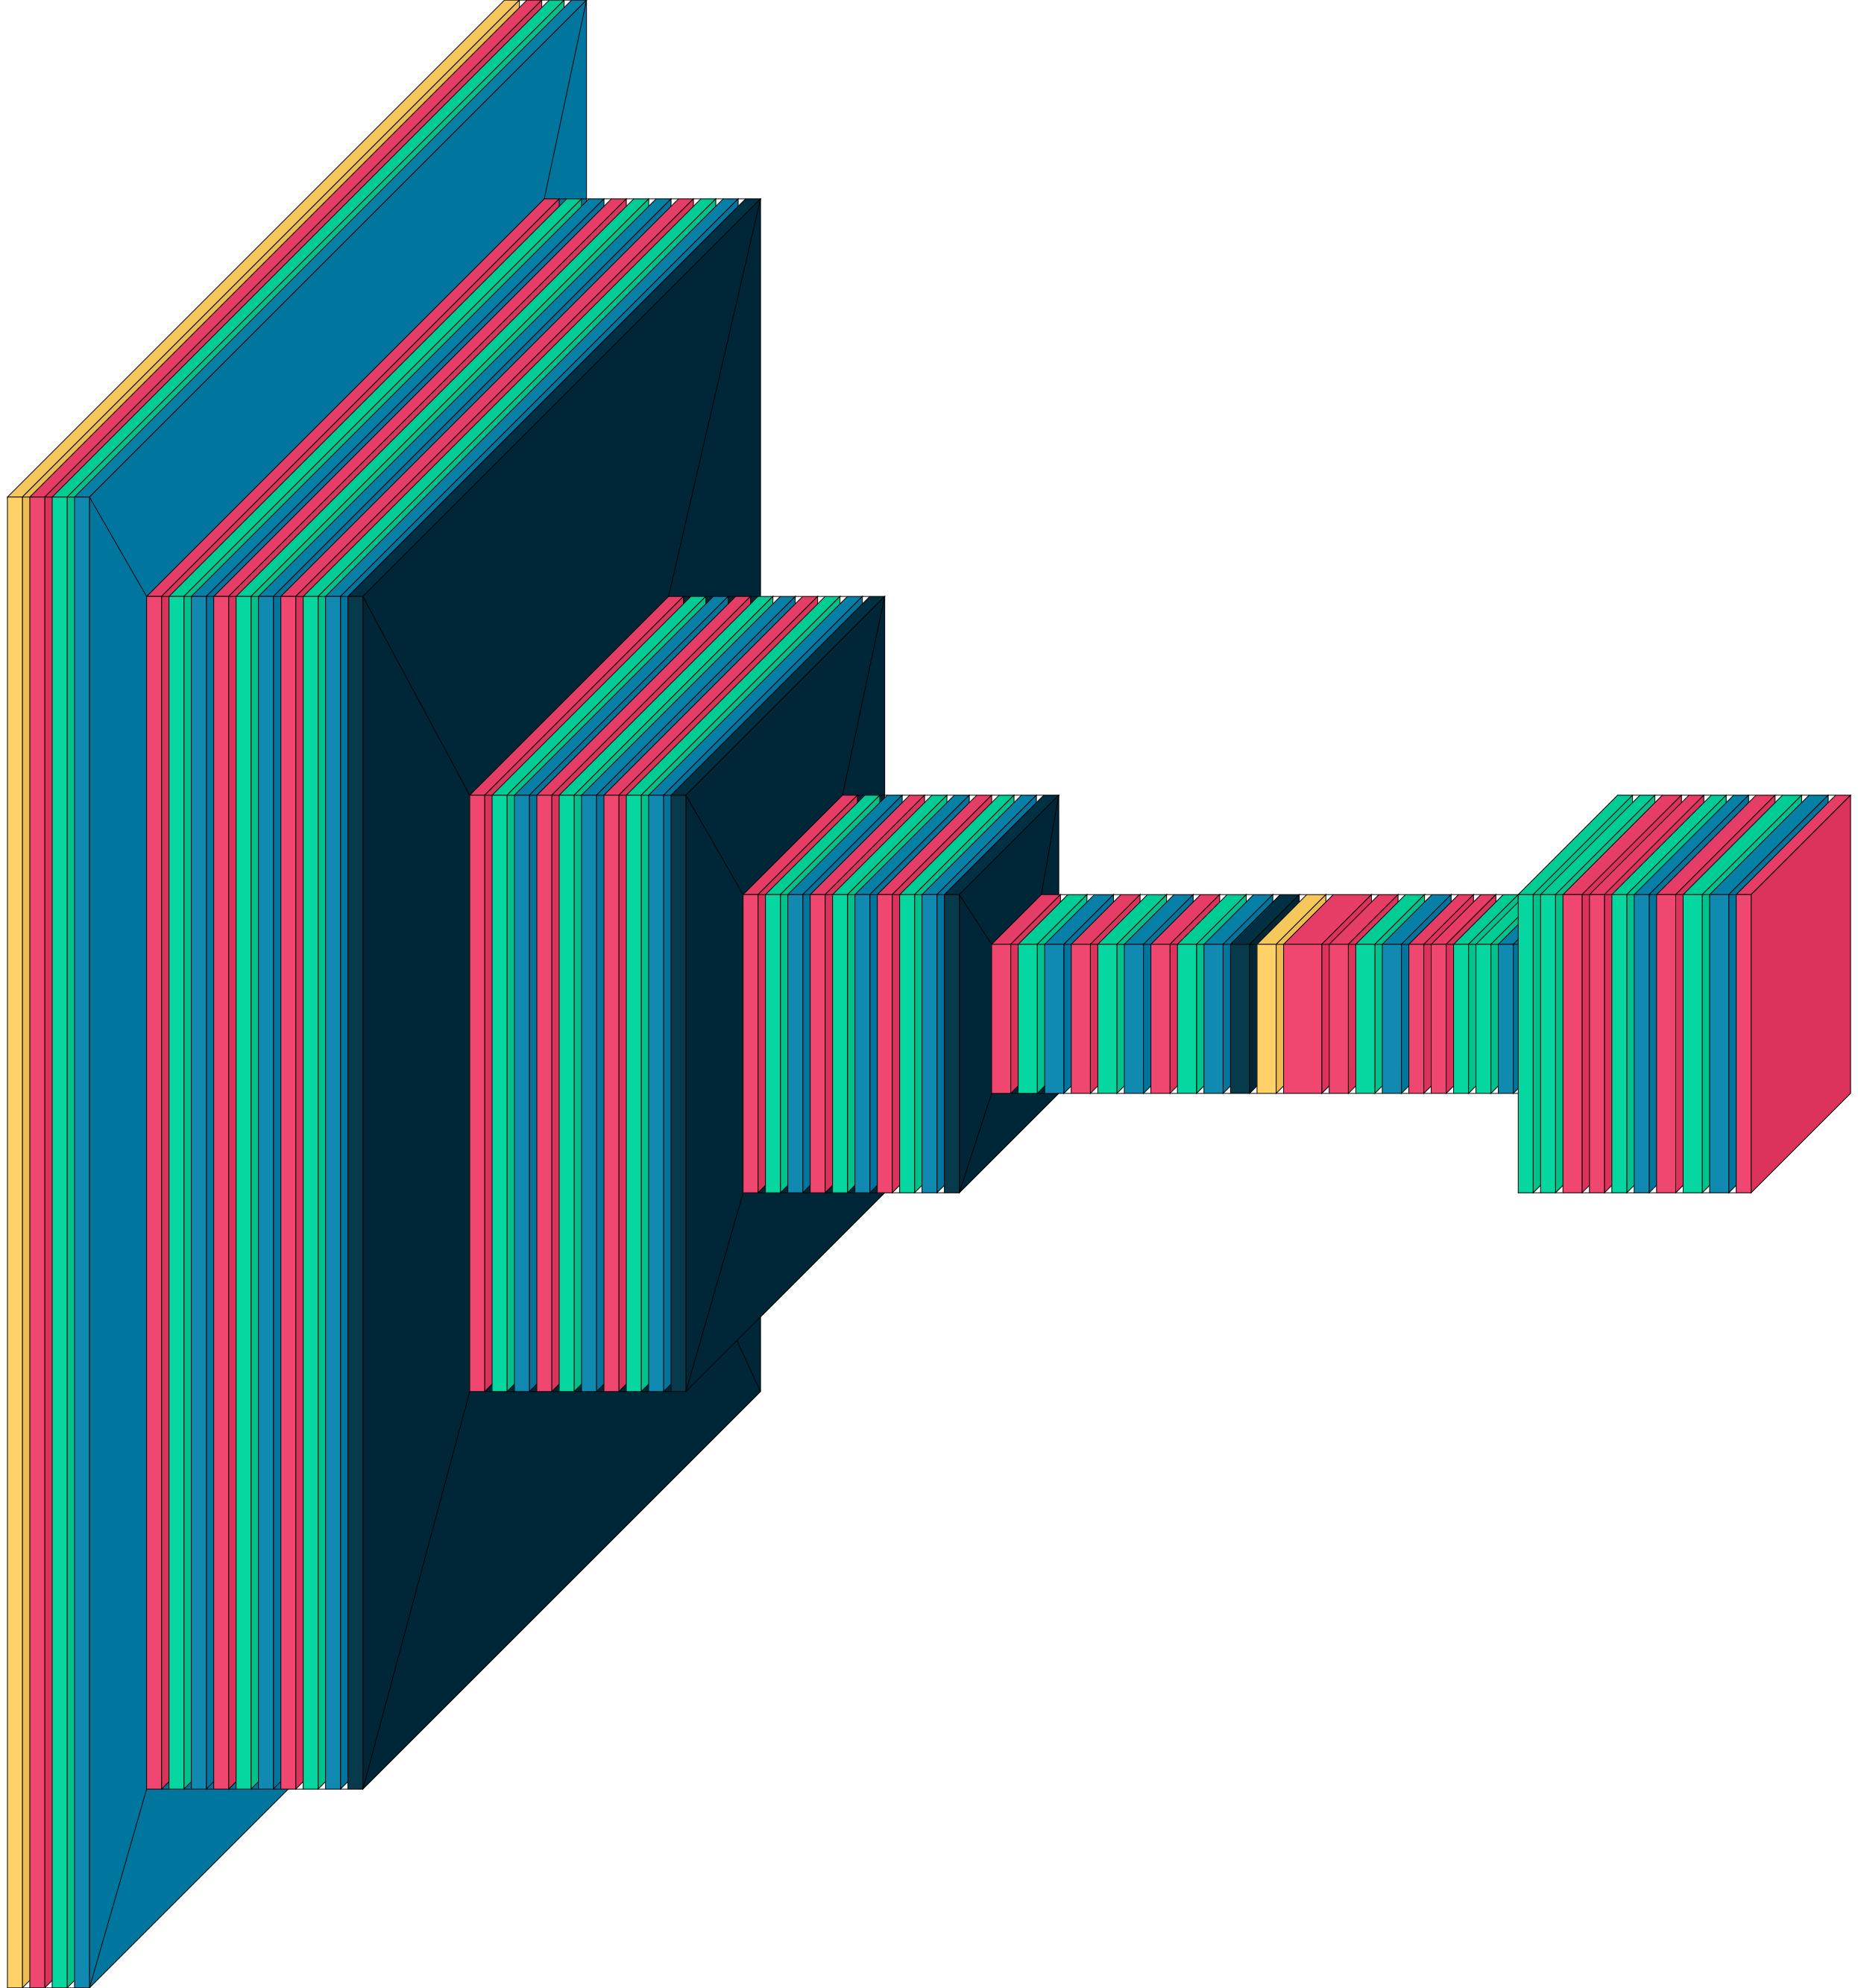
\includegraphics[scale=0.06]{gambar/yolov8_architecture_custom.png}
  % Change with the desired image caption
  \caption{Visualization with VisualKeras}
  \label{fig:YoloV8 Architecture Visualization with VisualKeras}
\end{figure}


\sloppy

YoloV8 uses Convolutional Neural Networks (CNN) as the basis of its architecture. In YOLO, CNN is used to extract features from the input image and then apply another network to predict Bounding Boxes and object classes directly from the image.

Based on one of the training sessions, this model has 225 layers, 3011043 parameters, and 8.2 GFLOPs. There are 2D Convolutional layers (Conv2D), C2f blocks, SPPF blocks, UpSampling layers, and Concatenate layers. Figure \ref{fig:YoloV8 IO Architecture} represents each type of layer with input and output.

\begin{figure}[H]
  \centering
  % Change with the desired image file name and size
  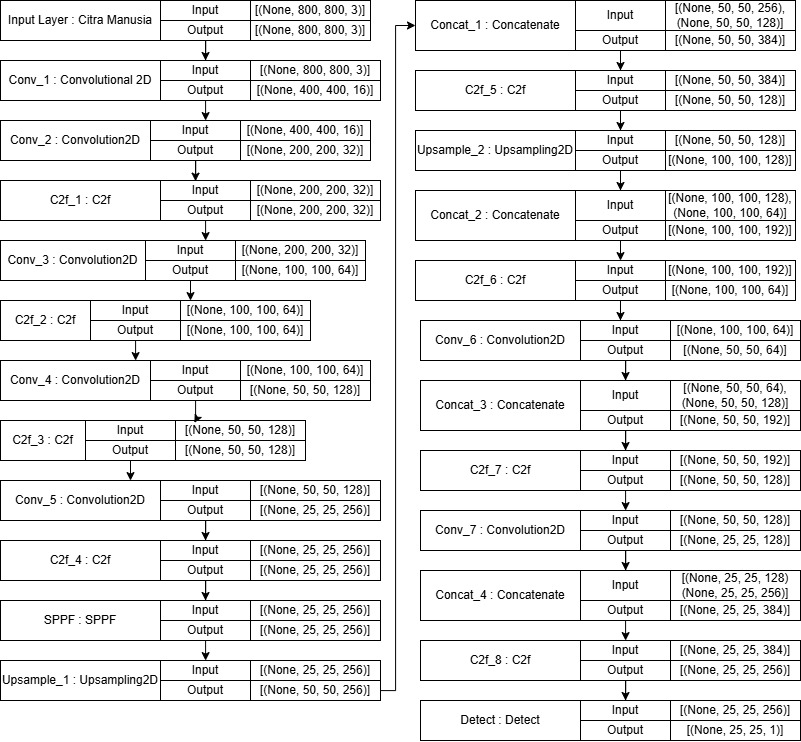
\includegraphics[scale=0.24]{gambar/Arsitektur.jpg}
  % Change with the desired image caption
  \caption{YoloV8 IO Architecture}
  \label{fig:YoloV8 IO Architecture}
\end{figure}

\subsection{MediaPipe Pose Estimation}
In this research, some relevant landmarks are keypoints on the elbows, forearms, and right and left shoulders. These keypoints were chosen based on their visibility and consistency in detection. Table \ref{tb:Keypoint Table} shows the keypoint numbers and names used in pose estimation.

\begin{table}[ht]
  \centering
  \caption{Keypoint Table}
  \label{tb:Keypoint Table}
  \begin{tabular}{|c|c|}
    \hline
    \rowcolor[HTML]{C0C0C0}
    \textbf{Keypoint Number} & \textbf{Keypoint Name} \\
    \hline
    11 & RIGHT\_SHOULDER \\
    12 & LEFT\_SHOULDER \\
    14 & RIGHT\_ELBOW \\
    16 & RIGHT\_WRIST \\
    \hline
  \end{tabular}
\end{table}


\subsection{Distance Calculation}
One way to calculate distance using a bounding box is through the concept of \emph{focal length pixel} ($f_p$). Focal length in pixels, or \emph{focal length pixel}, is the conversion of the camera lens's focal length, usually measured in millimeters, into pixels. This is a key concept in photogrammetry and computer vision used to relate visual information from the camera to physical size in the real world.

In the context of this thesis, focal length in pixels is used to convert the obstacle size from pixel units to meter units. This is important because the autonomous wheelchair needs to understand the actual distance to obstacles to make accurate navigation decisions. The formula can be seen in Equation \ref{eq:fp formula}:

\begin{equation}
\label{eq:fp formula}
f_p = \frac{D \times h_b}{H_o}
\end{equation}

Where:
\begin{itemize}
\item $f_p$ is the focal length in pixels,
\item $D$ is the actual distance from the camera to the object,
\item $h_b$ is the height of the bounding box in pixels,
\item $H_o$ is the actual height of the object.
\end{itemize}

When calculating the distance to an object, the detected bounding box height by YOLO is used, combined with the known actual height of the object and the focal length in pixels. This forms Equation \ref{eq:Distance Formula} as follows:

\begin{equation}
\label{eq:Distance Formula}
D = \frac{f_p \times H_o}{h_b}
\end{equation}

Here:
\begin{itemize}
\item $H_o$ is the average height of a human or other identified object.
\end{itemize}

Another approach in determining distance using pose is through the Euclidean Distance method. Euclidean Distance in pixels is a method to measure the straight-line distance between two points in image space, usually measured in pixels. In the context of this thesis, which involves an autonomous wheelchair with MediaPipe integration, this measurement is crucial for various functions, especially in pose analysis and assessing the proportion of objects in the images produced by the camera. The formula can be seen in Equation \ref{eq:Euclidean Distance}

\begin{equation}
\label{eq:Euclidean Distance}
d_p = \sqrt{(x_2 - x_1)^2 + (y_2 - y_1)^2} \times s_f
\end{equation}

Where:
\begin{itemize}
\item $d_p$ is the Euclidean distance in pixels,
\item $(x_1, y_1)$ and $(x_2, y_2)$ are the coordinates of two points measured in pixels,
\item $s_f$ is the scale factor.
\end{itemize}

This formula yields the distance between two points in the same units as the coordinates $x_1, y_1$, and $x_2, y_2$. Typically, if these coordinates are measured in pixels, the resulting distance will also be in pixels.

From the above calculations, the distance is still in pixel units. In the context of distance calculation, a standard value in meters is needed to align with general measurement standards. To convert these pixel values into meters, calibration using the value \emph{K} is necessary. The value \emph{K} is a calibration value based on experimental measurements. Equation \ref{eq:Distance Constant} is as follows:

\begin{equation}
\label{eq:Distance Constant}
D_m = \left(\frac{K}{{d_p}}\right)
\end{equation}

Where:
\begin{itemize}
\item $D_m$ is the distance in meters,
\item $K$ is the calibration constant,
\item $d_p$ is the distance in pixels.
\end{itemize}

The value \emph{K} determines how much influence the pixel distance has on the meter distance. Larger or smaller values will directly affect the distance calculation results. For example, a larger \emph{K} value will result in a smaller distance for the same number of pixels. This value is used in a very specific context where this parameter describes the direct relationship between pixel size and actual distance or dimensions, based on specific assumptions about the scene's geometry and camera characteristics.

This value must be accurately calibrated to match the specific characteristics of the camera and setup used. Incorrect calibration will result in inaccurate distance measurements, which can impact the autonomous wheelchair's navigation decisions. The calibration formula for the \emph{K} value using Equation \ref{eq:K value} is as follows:

\begin{equation}
\label{eq:K value}
K = J_o \times U_p
\end{equation}

Where:
\begin{itemize}
\item $J_o$ is the actual object distance,
\item $U_p$ is the object size in pixels.
\end{itemize}

In the calculation of obstacle width, the Euclidean distance calculation is used but with a different application context. Both approaches differ in application and context. The differences can be seen in Equation \ref{eq:Euclidean Width2}

\begin{equation}
\label{eq:Euclidean Width2}
l_p = \sqrt{(x_2 - x_1)^2 + (y_2 - y_1)^2} \times s_f
\end{equation}

The output value obtained is the width of the human in pixels. To map the width from pixels to meters, a conversion formula is needed to determine the size in pixels (which is a digital and relative size) to real-world size (meters). The formula can be seen in Equation \ref{eq:Width Meter2}:

\begin{equation}
\label{eq:Width Meter2}
l_m = l_p \times s_f
\end{equation}

By multiplying the object's width in pixels by the scale factor, the result is the object's width in meters. This formula is useful in applications where the real-world dimensions of objects need to be known to make accurate decisions or measurements.

The scale factor is a value that converts the size from pixel units to meter units. This value is obtained through the calibration process. The scale factor determines how many meters are represented by each pixel in the image, based on the camera's distance to the object and other camera settings such as focal length. Additionally, note that the scale factor used in this formula differs from the distance formula previously explained. The calibration formula for the scale factor in the context of object width in Equation \ref{eq:scale factor2} is as follows:

\begin{equation}
\label{eq:scale factor2}
s_f = \frac{D_n}{U_p}
\end{equation}

Where:
\begin{itemize}
\item $D_n$ is the average actual dimension,
\item $U_p$ is the average size in pixels.
\end{itemize}

In the calculation of obstacle width, the Euclidean distance calculation is used but with a different application context. Both approaches differ in application and context. The differences can be seen in Equation \ref{eq:Euclidean Width}

\begin{equation}
\label{eq:Euclidean Width}
l_p = \sqrt{(x_2 - x_1)^2 + (y_2 - y_1)^2} \times s_f
\end{equation}

The output value obtained is the width of the human in pixels. To map the width from pixels to meters, a conversion formula is needed to determine the size in pixels (which is a digital and relative size) to real-world size (meters). The formula can be seen in Equation \ref{eq:Width Meter}:

\begin{equation}
\label{eq:Width Meter}
l_m = l_p \times s_f
\end{equation}

By multiplying the object's width in pixels by the scale factor, the result is the object's width in meters. This formula is useful in applications where the real-world dimensions of objects need to be known to make accurate decisions or measurements.

The scale factor is a value that converts the size from pixel units to meter units. This value is obtained through the calibration process. The scale factor determines how many meters are represented by each pixel in the image, based on the camera's distance to the object and other camera settings such as focal length. Additionally, note that the scale factor used in this formula differs from the distance formula previously explained. The calibration formula for the scale factor in the context of object width in Equation \ref{eq:scale factor} is as follows:

\begin{equation}
\label{eq:scale factor}
s_f = \frac{D_n}{U_p}
\end{equation}

Where:
\begin{itemize}
\item $D_n$ is the average actual dimension,
\item $U_p$ is the average size in pixels.
\end{itemize}

These values can be used in the code to convert sizes from pixels to real sizes based on calibrated measurements. Calibration must be done correctly to obtain accurate results.

\subsection{Grid Implementation}
In this thesis, the autonomous wheelchair must be able to determine the position of obstacles it will encounter. Therefore, a map is needed as a reference for the wheelchair to take action based on the obstacle distance and width, which will be used to determine where the wheelchair should avoid and whether the obstacle has been successfully avoided. Grid is one of the best approaches in mapping detection results. Using a grid not only facilitates decision-making but also provides easy-to-understand visualization. The grid size can also be adjusted according to needs, both in dimensions and appearance.

After the above formulas are implemented in the code, several important variables will be obtained to be used in mapping the position and size of obstacles in the grid. Before that, here is the grid used, as shown in Figure \ref{fig:Grid10x10}:

\begin{figure}[H]
  \centering
  % Change with the desired image file name and size
  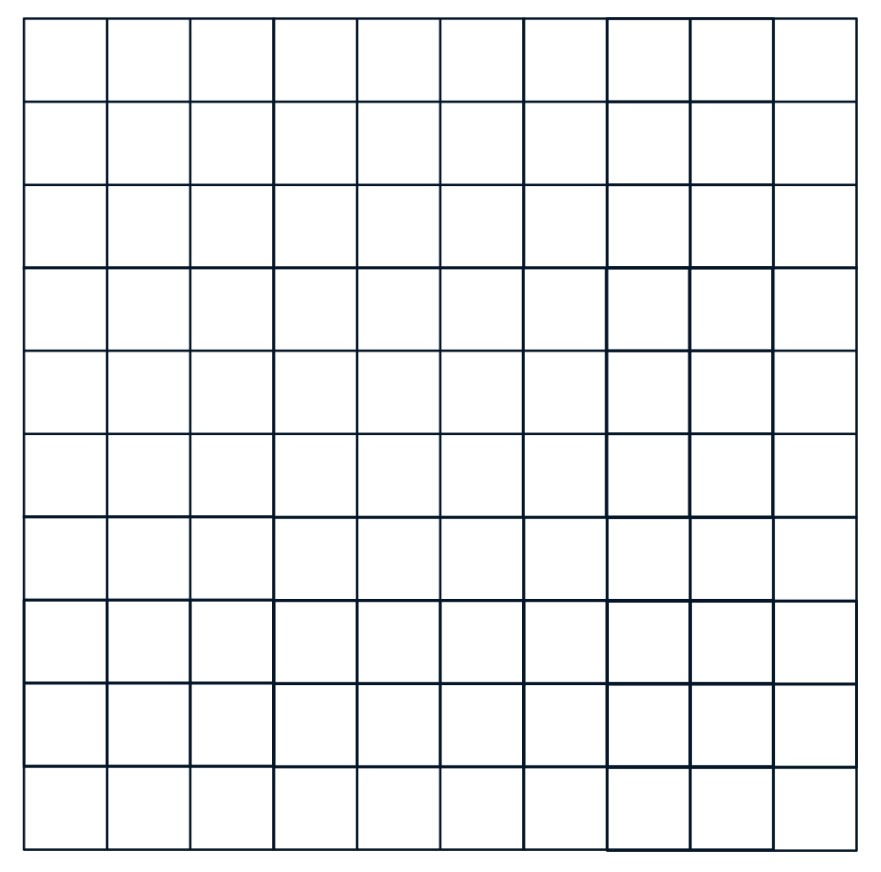
\includegraphics[scale=0.2]{gambar/gridtanpakamera2.jpg}
  % Change with the desired image caption
  \caption{10x10 Grid}
  \label{fig:Grid10x10}
\end{figure}

The grid is created using the OpenCV library. This library is chosen because of its easy and lightweight implementation. For better understanding, the explanation will be accompanied by a 3D visualization using Blender in Figure \ref{fig:gridxblendxmanusiatengah}.

\begin{figure}[H]
  \centering
  % Change with the desired image file name and size
  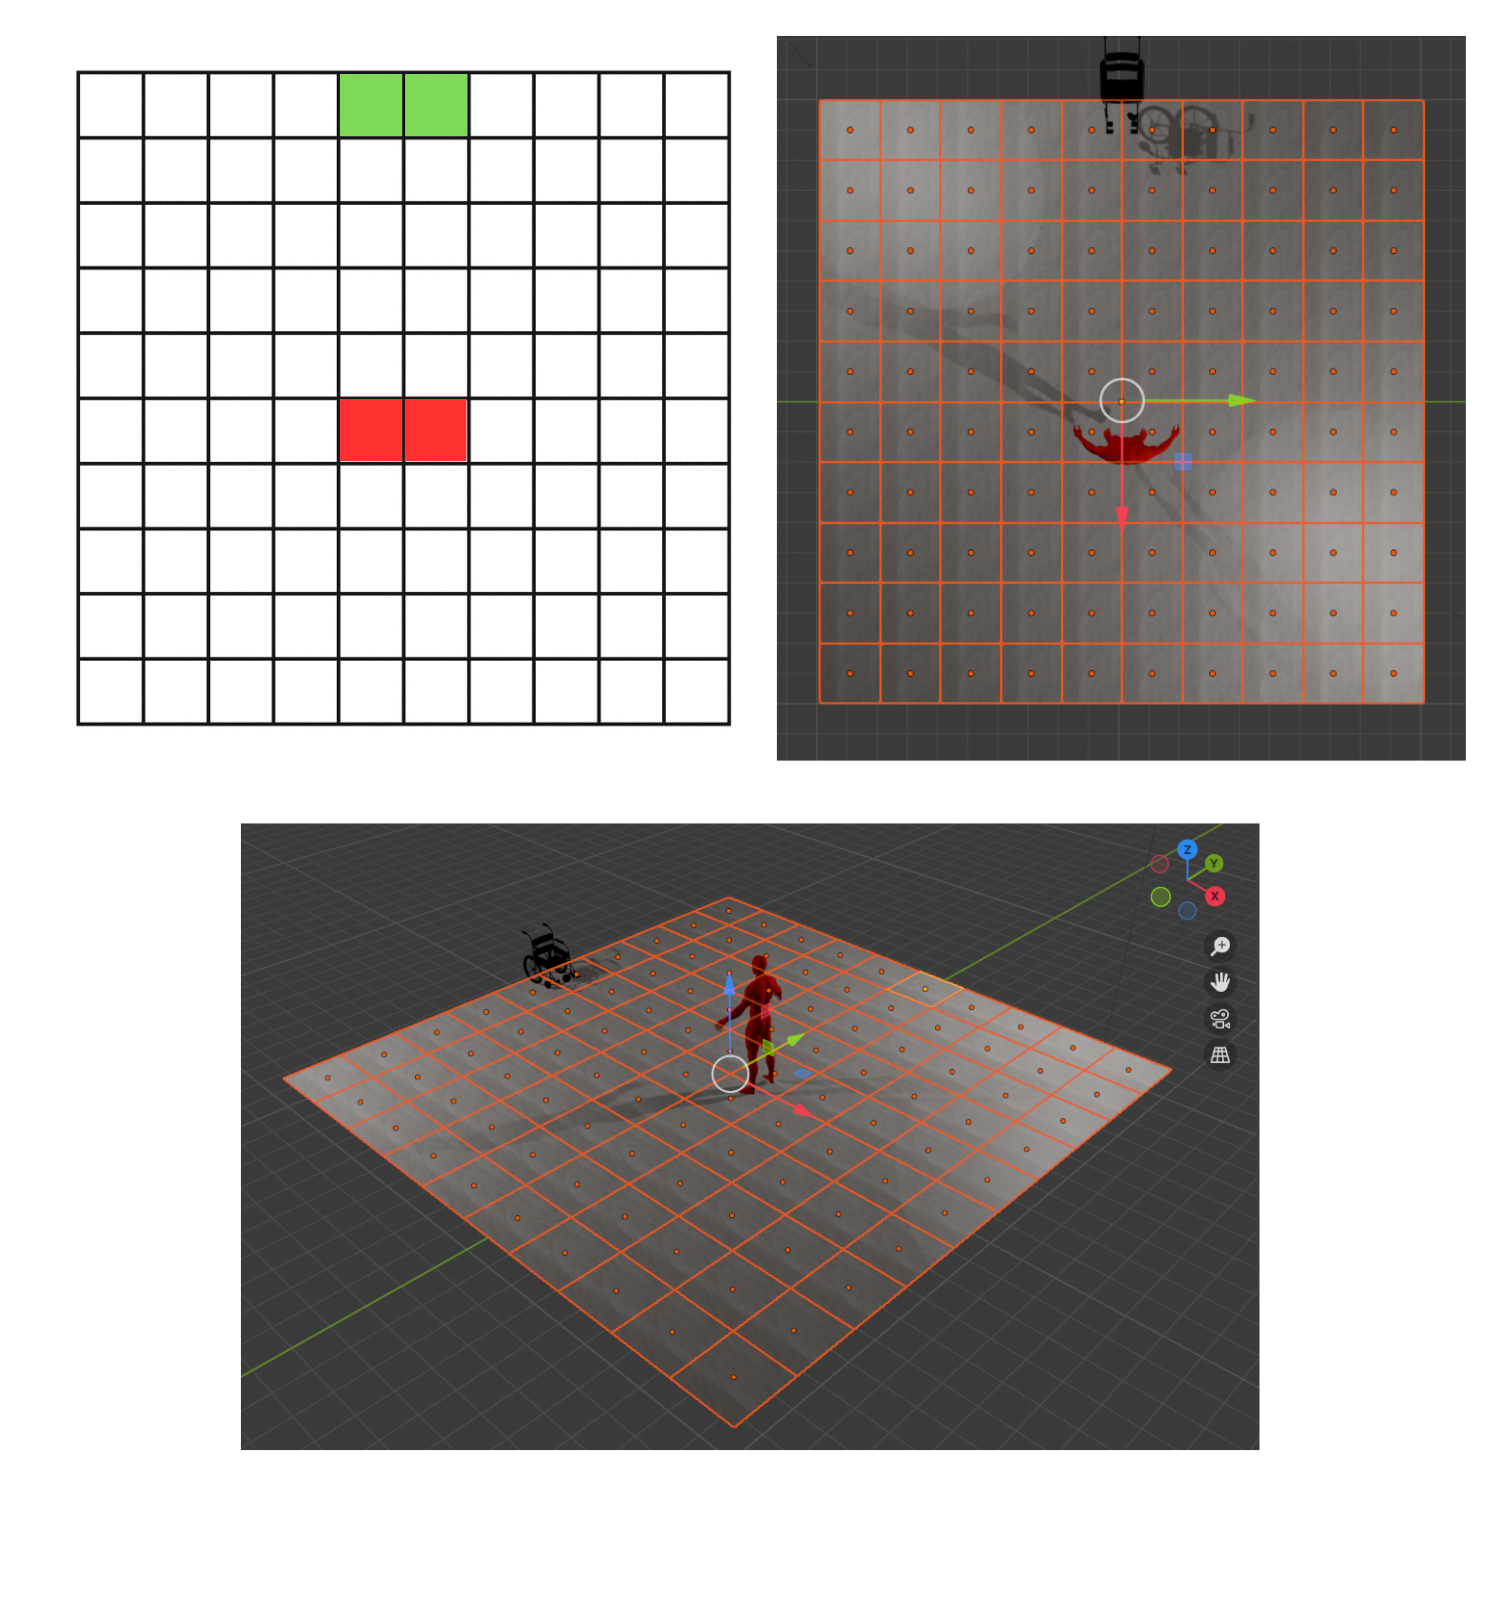
\includegraphics[scale=0.15]{gambar/elbaruelbaru.png}
  % Change with the desired image caption
  \caption{Grid Visualization with Blender}
  \label{fig:gridxblendxmanusiatengah}
\end{figure}


The use of a 10x10 grid is based on image results and model performance. Both bounding boxes and poses have limitations where their calculation results do not exceed the parameters set on the grid. These parameters can be seen in Figure \ref{fig:Grid Parameters}:

\begin{figure}[H]
  \centering
  % Change with the desired image file name and size
  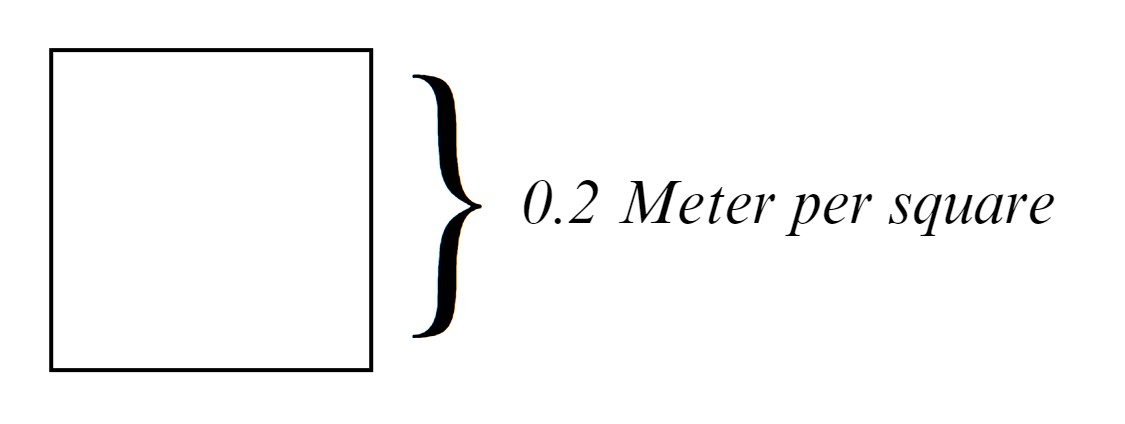
\includegraphics[scale=0.2]{gambar/02meter.jpg}
  % Change with the desired image caption
  \caption{Parameters for each grid box}
  \label{fig:Grid Parameters}
\end{figure}

From the above image, each box in the grid is 0.2 meters in both vertical and horizontal positions. The determination of 0.2 meters per box is based on calibration and experimental measurements ensuring this size is optimal for accurate and efficient obstacle detection.

To map objects well in the grid, an index must be created to determine the object's relative left and right positions to the camera. For 10 horizontal boxes, they will be divided into left and right indices, where indices 1 to 5 are categorized as left indices, and indices 6 to 10 are categorized as right indices. This decision is related to the static wheelchair position on the grid, depicted in Figure \ref{fig:Wheelchair Position on Grid}:

\begin{figure}[H]
  \centering
  % Change with the desired image file name and size
  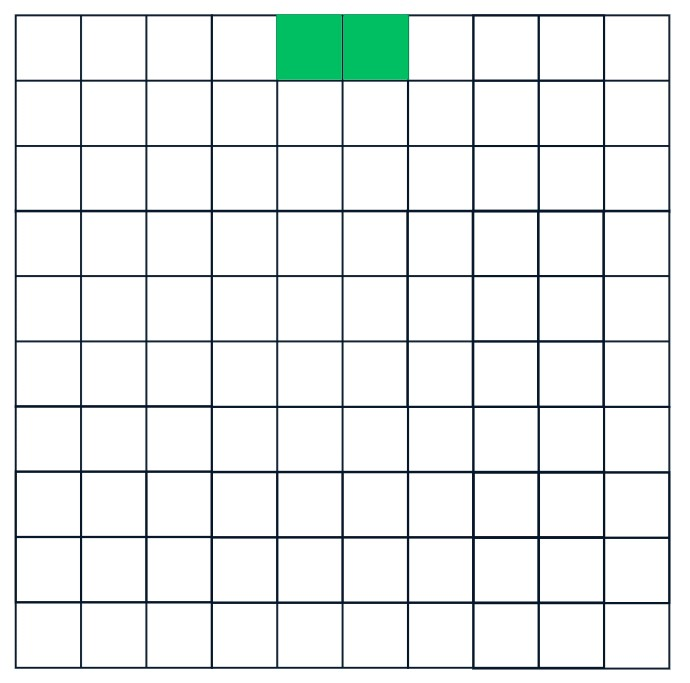
\includegraphics[scale=0.2]{gambar/gridkamera.jpg}
  % Change with the desired image caption
  \caption{Wheelchair Position on Grid}
  \label{fig:Wheelchair Position on Grid}
\end{figure}

It can be seen that the wheelchair position occupies 2 green grid boxes at (5,1) and (6,1). This decision is based on the wheelchair's width, which fits the grid size. The top position determines which indices are left and right on the grid. With the top position set as the wheelchair's constant position and the input image results obtained as mirrored detection results, the indices can be depicted according to Figure \ref{fig:Position Categories based on Index}:

\begin{figure}[H]
  \centering
  % Change with the desired image file name and size
  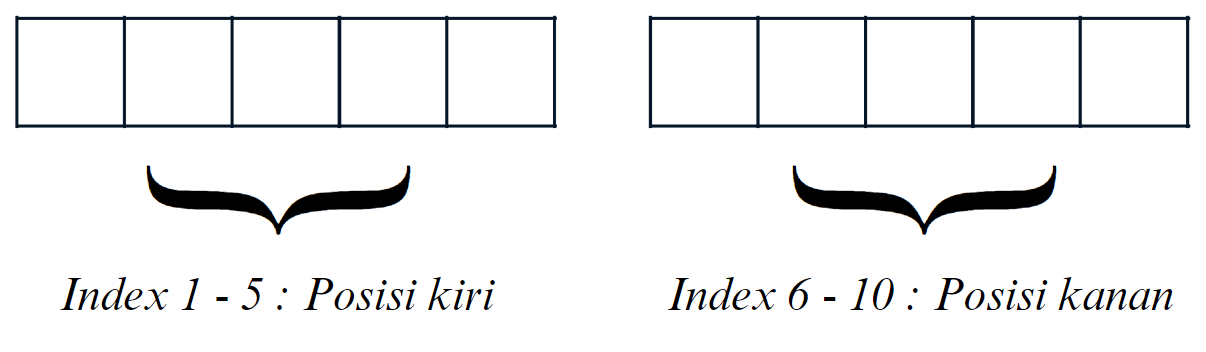
\includegraphics[scale=0.2]{gambar/posisi index sebenarnya.png}
  % Change with the desired image caption
  \caption{Position Categories based on Index}
  \label{fig:Position Categories based on Index}
\end{figure}

This categorization plays an important role in the wheelchair's turn decision-making, where the detection results in the form of distance, width, and relative position will be displayed on the grid.

\subsection{Wheelchair Avoidance Navigation}

\subsubsection{Results without Detection}
In this condition, no objects are detected, meaning there are no obstacles blocking the wheelchair's path, so the wheelchair will continue to move forward. In this condition, the bounding box, pose, grid, and others are not displayed because no humans are detected. It can be seen in the example image \ref{fig:Condition without detection}

\begin{figure}[H]
    \centering
    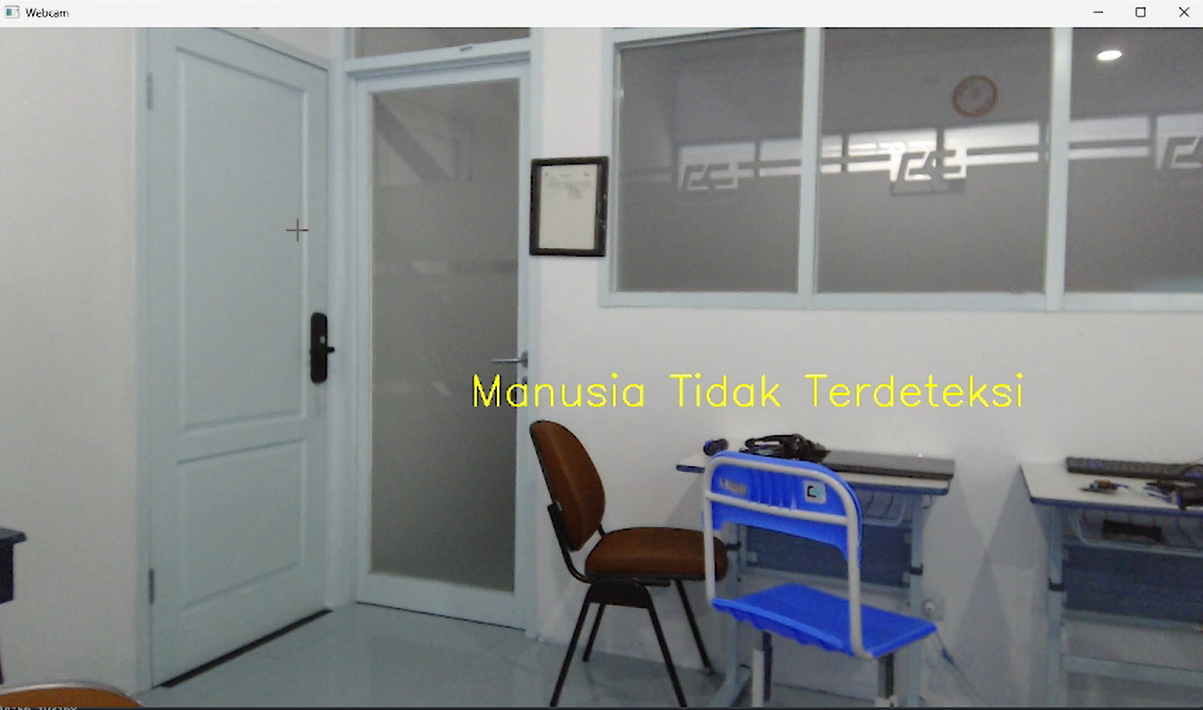
\includegraphics[scale=0.2]{gambar/masukinkebuku.png}
    \caption{Example condition without Human Detection}
    \label{fig:Condition without detection}
\end{figure}

It can be seen in Figure \ref{fig:Condition without detection}, there is text "No Humans Detected," which means no human objects are detected.

\subsubsection{Object detection results on the grid showing Left Index greater
than Right Index}
In this condition, the detection result position shows a higher value on the left index (indices 1-5), meaning the object is on the left side relative to the wheelchair position. This can be seen in the example image below.

\begin{figure}[H]
  \centering
  % Change with the desired image file name and size
  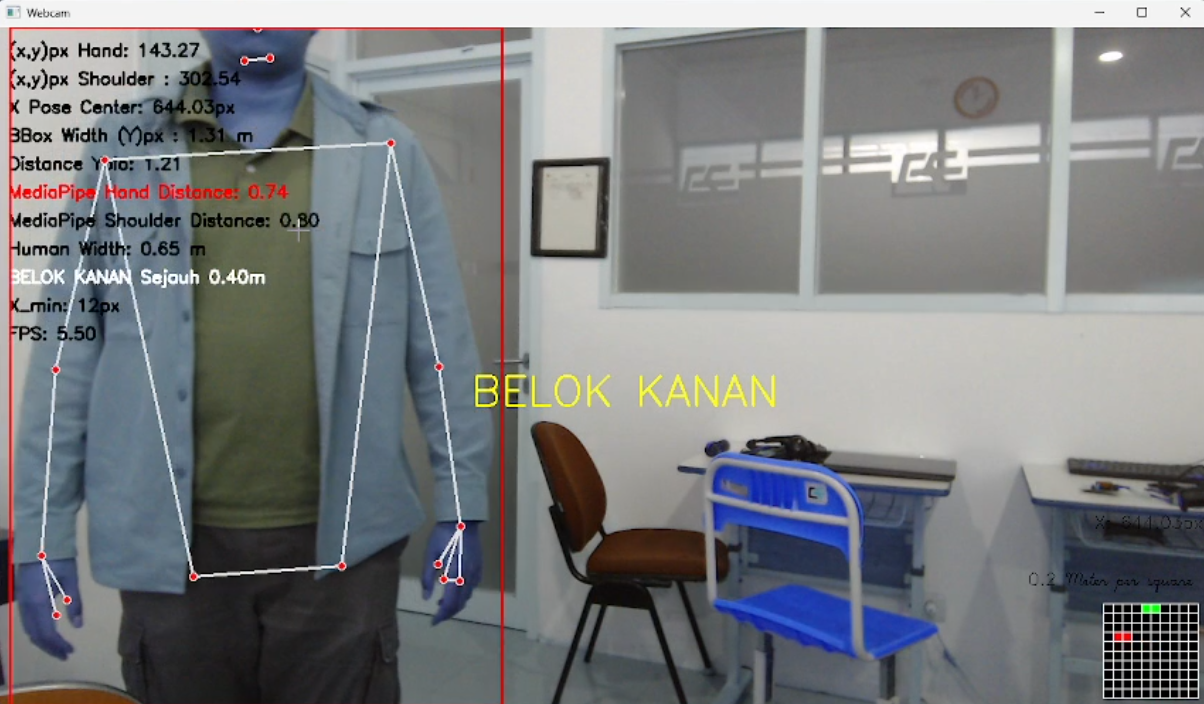
\includegraphics[scale=0.2]{gambar/BelokKananbos.png}
  % Change with the desired image caption
  \caption{Example condition Left Index \textgreater Right}
  \label{fig:Condition Left Index > Right}
\end{figure}

It can be seen in Figure \ref{fig:Condition Left Index > Right}, the grid value is more towards the left index than the right. Based on this position, the wheelchair will avoid to the right, which is a safer turn than to the left.

The wheelchair can only be said to avoid if it returns to its original direction. Thus, Figure \ref{fig:Scheme Condition Left Index > Right} is the avoidance scheme that will be followed in this condition.

\begin{figure}[H]
  \centering
  % Change with the desired image file name and size
  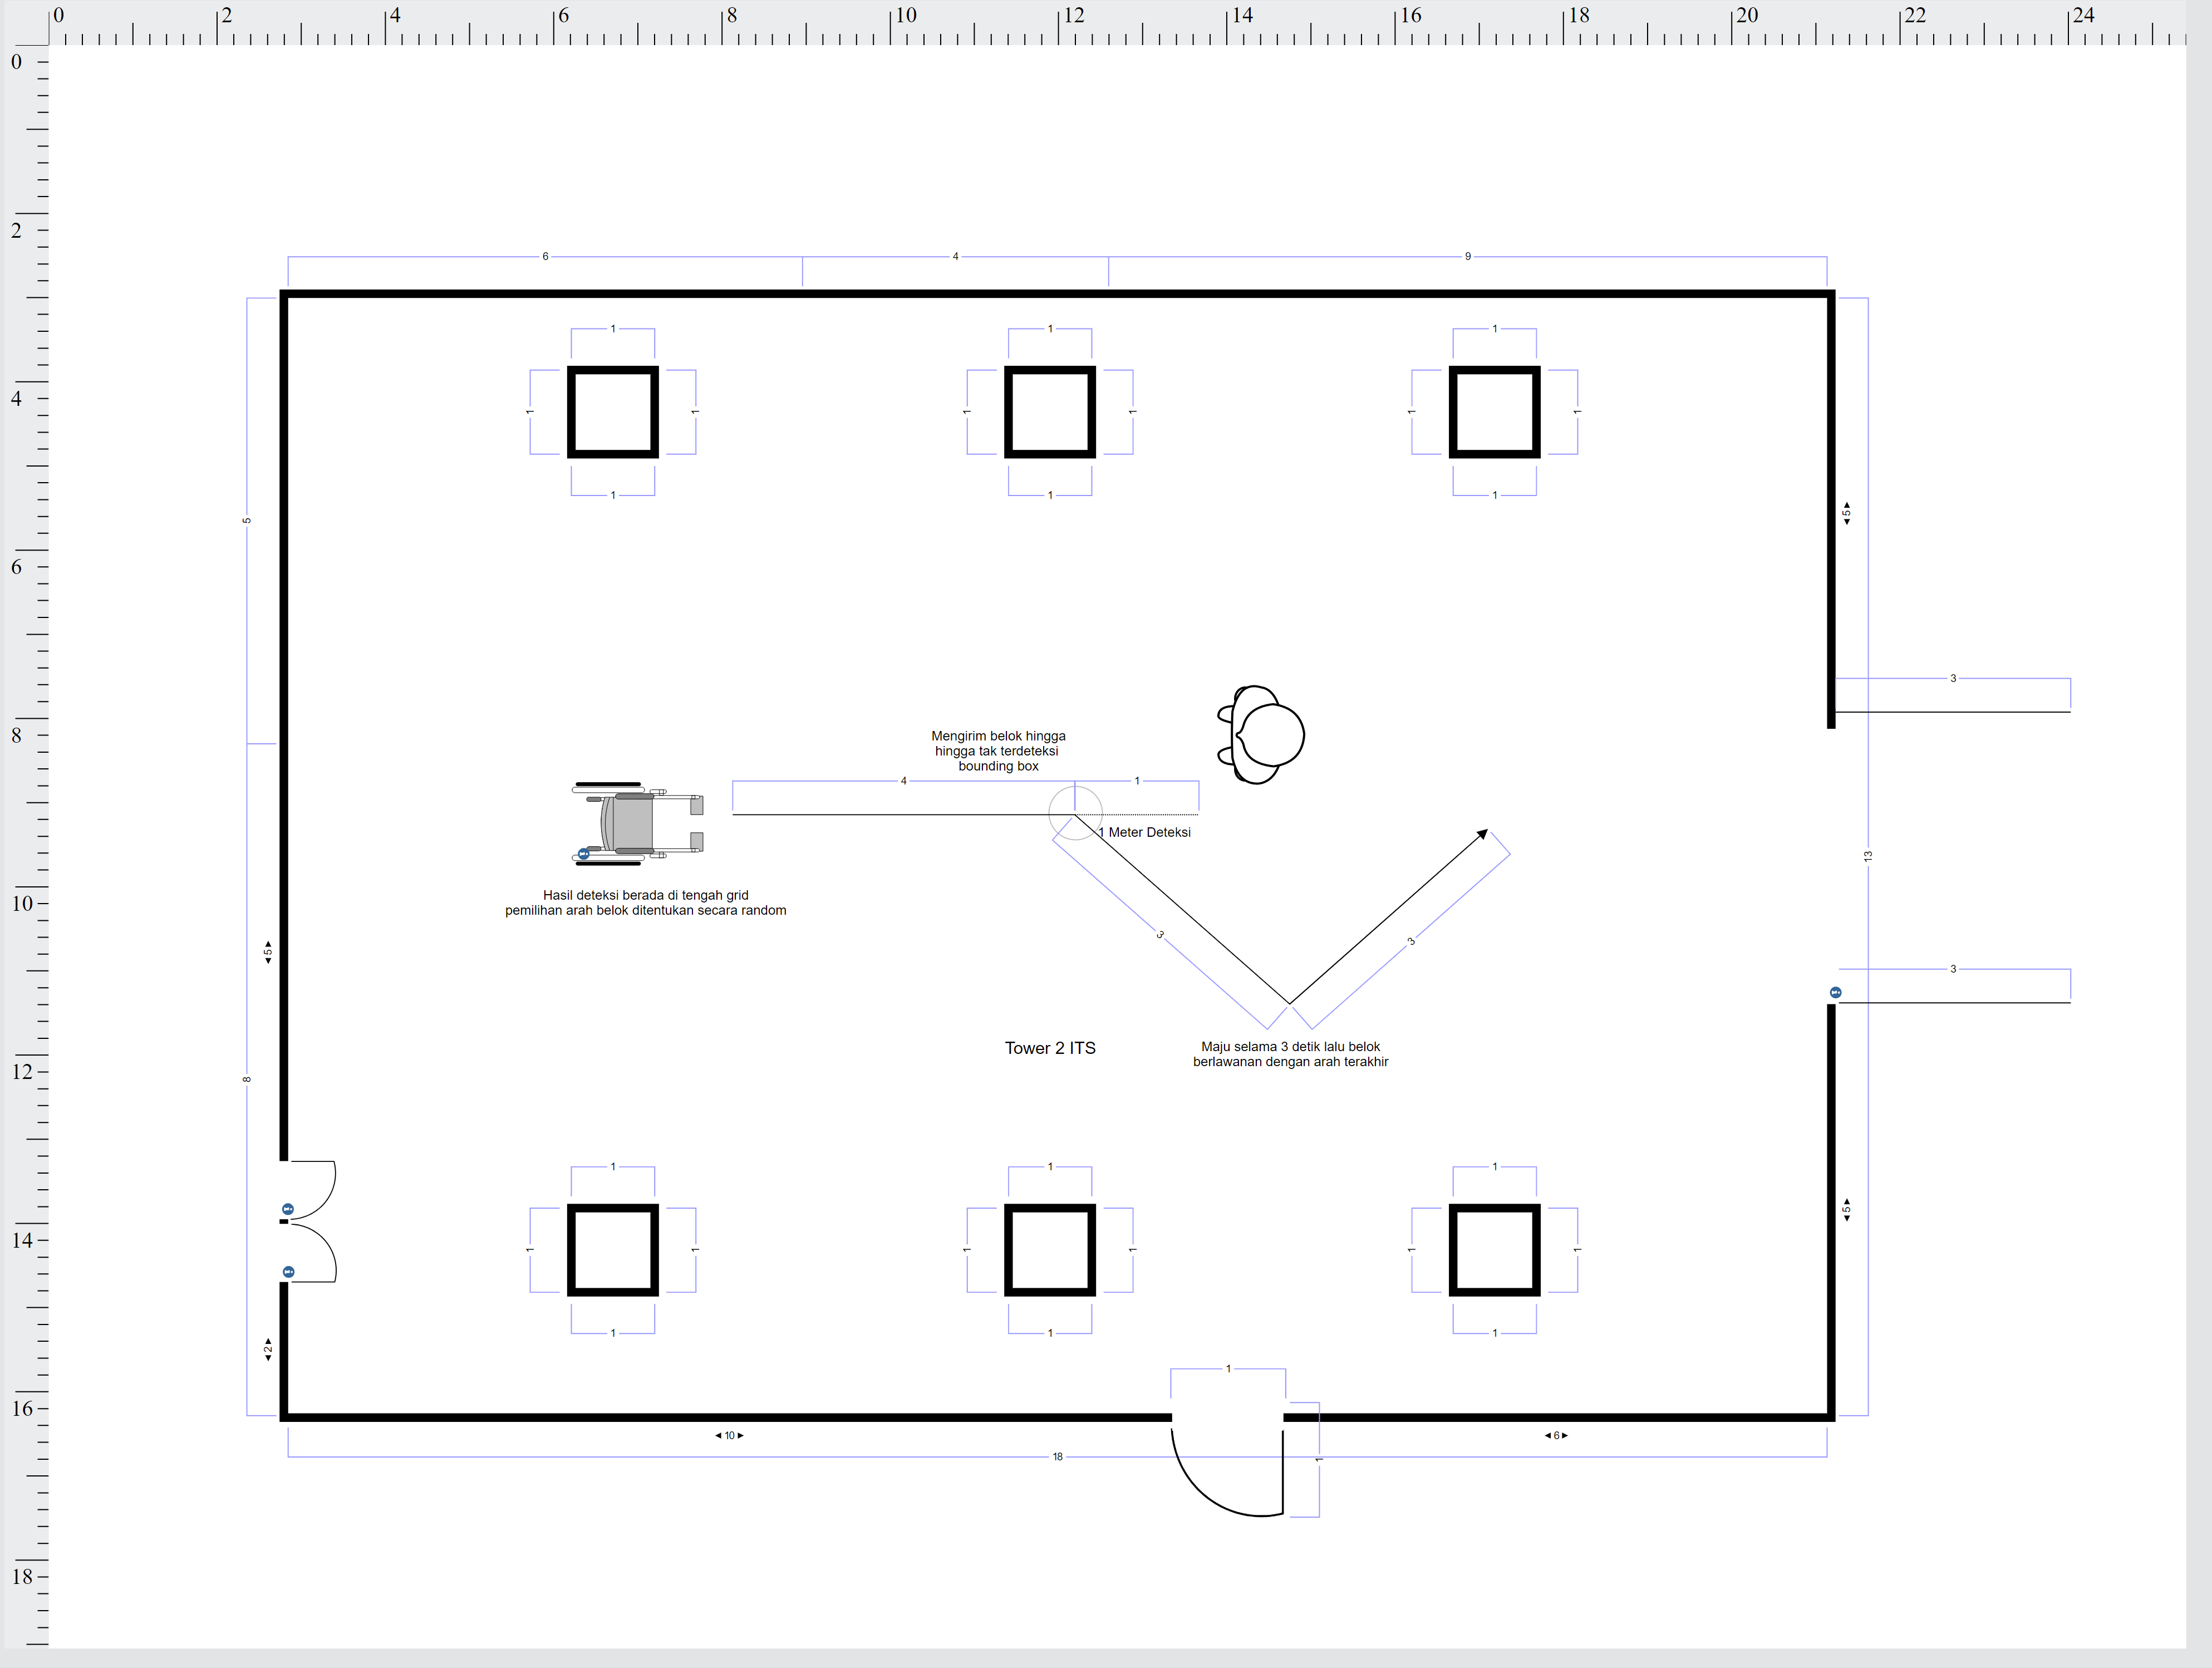
\includegraphics[scale=0.06]{gambar/ManusiaKiriNavigasi.png}
  % Change with the desired image caption
  \caption{Avoidance scheme in condition Left Index \textgreater Right}
  \label{fig:Scheme Condition Left Index > Right}
\end{figure}

It can be seen in Figure \ref{fig:Scheme Condition Left Index > Right} that when the wheelchair is 1 meter from detection, it will turn according to the index condition and store this turn direction. If the bounding box is no longer visible, the wheelchair will move forward for 4 seconds, then check the last turn direction. Then the wheelchair will turn again according to the last direction for 5 seconds, then reset the last direction condition. Finally, in this condition, the wheelchair will enter the no detection condition, so it will continue to move forward until the next detection.

\subsubsection{Object detection results on the grid showing the right index greater than the left index}

In this condition, the detection result position shows a higher value on the right index (6-10), meaning the object is on the right side relative to the wheelchair position. This can be seen in the example image \ref{fig:Condition Right Index > Left}

\begin{figure}[H]
    \centering
    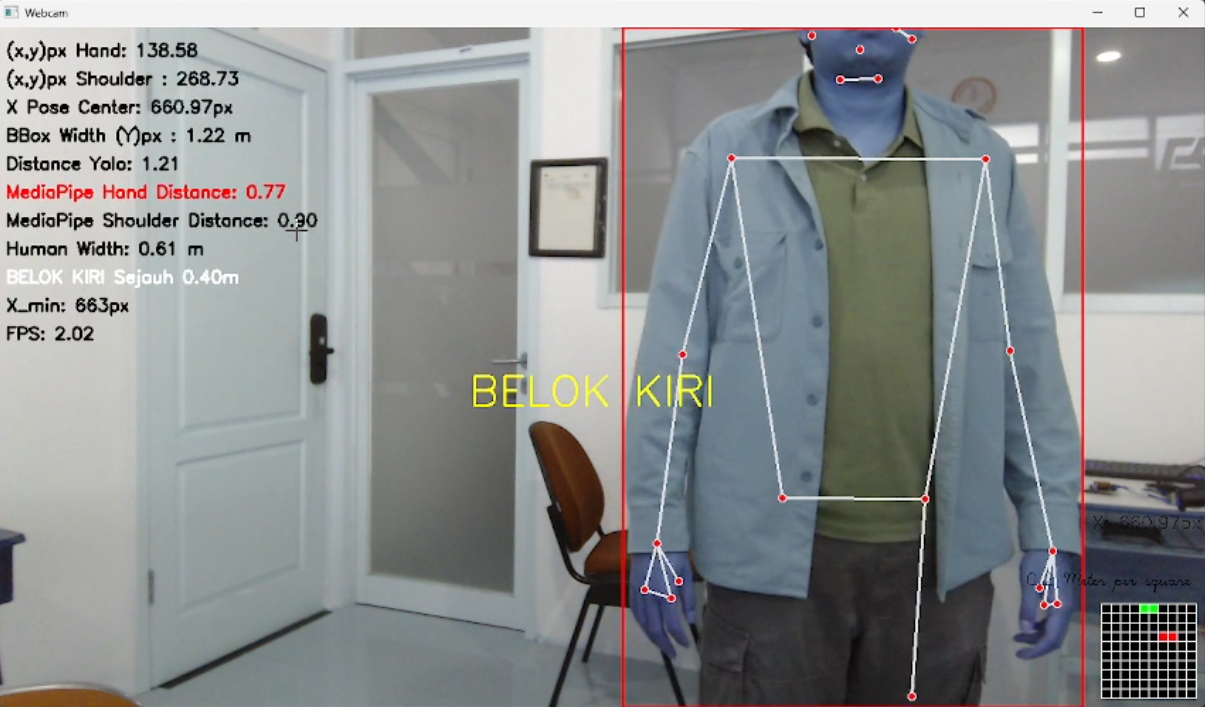
\includegraphics[scale=0.2]{gambar/BelokKiribos.png}
    \caption{Example condition Right Index \textgreater Left}
    \label{fig:Condition Right Index > Left}
\end{figure}

It can be seen in Figure \ref{fig:Condition Right Index > Left}, the grid value is more towards the right index than the left. Based on this position, the wheelchair will avoid to the left, which is a safer turn than to the right.

The wheelchair can only be said to avoid if it returns to its original direction. Thus, Figure \ref{fig:Scheme Condition Right Index > Left} is the avoidance scheme that will be followed in this condition.

\begin{figure}[H]
  \centering
  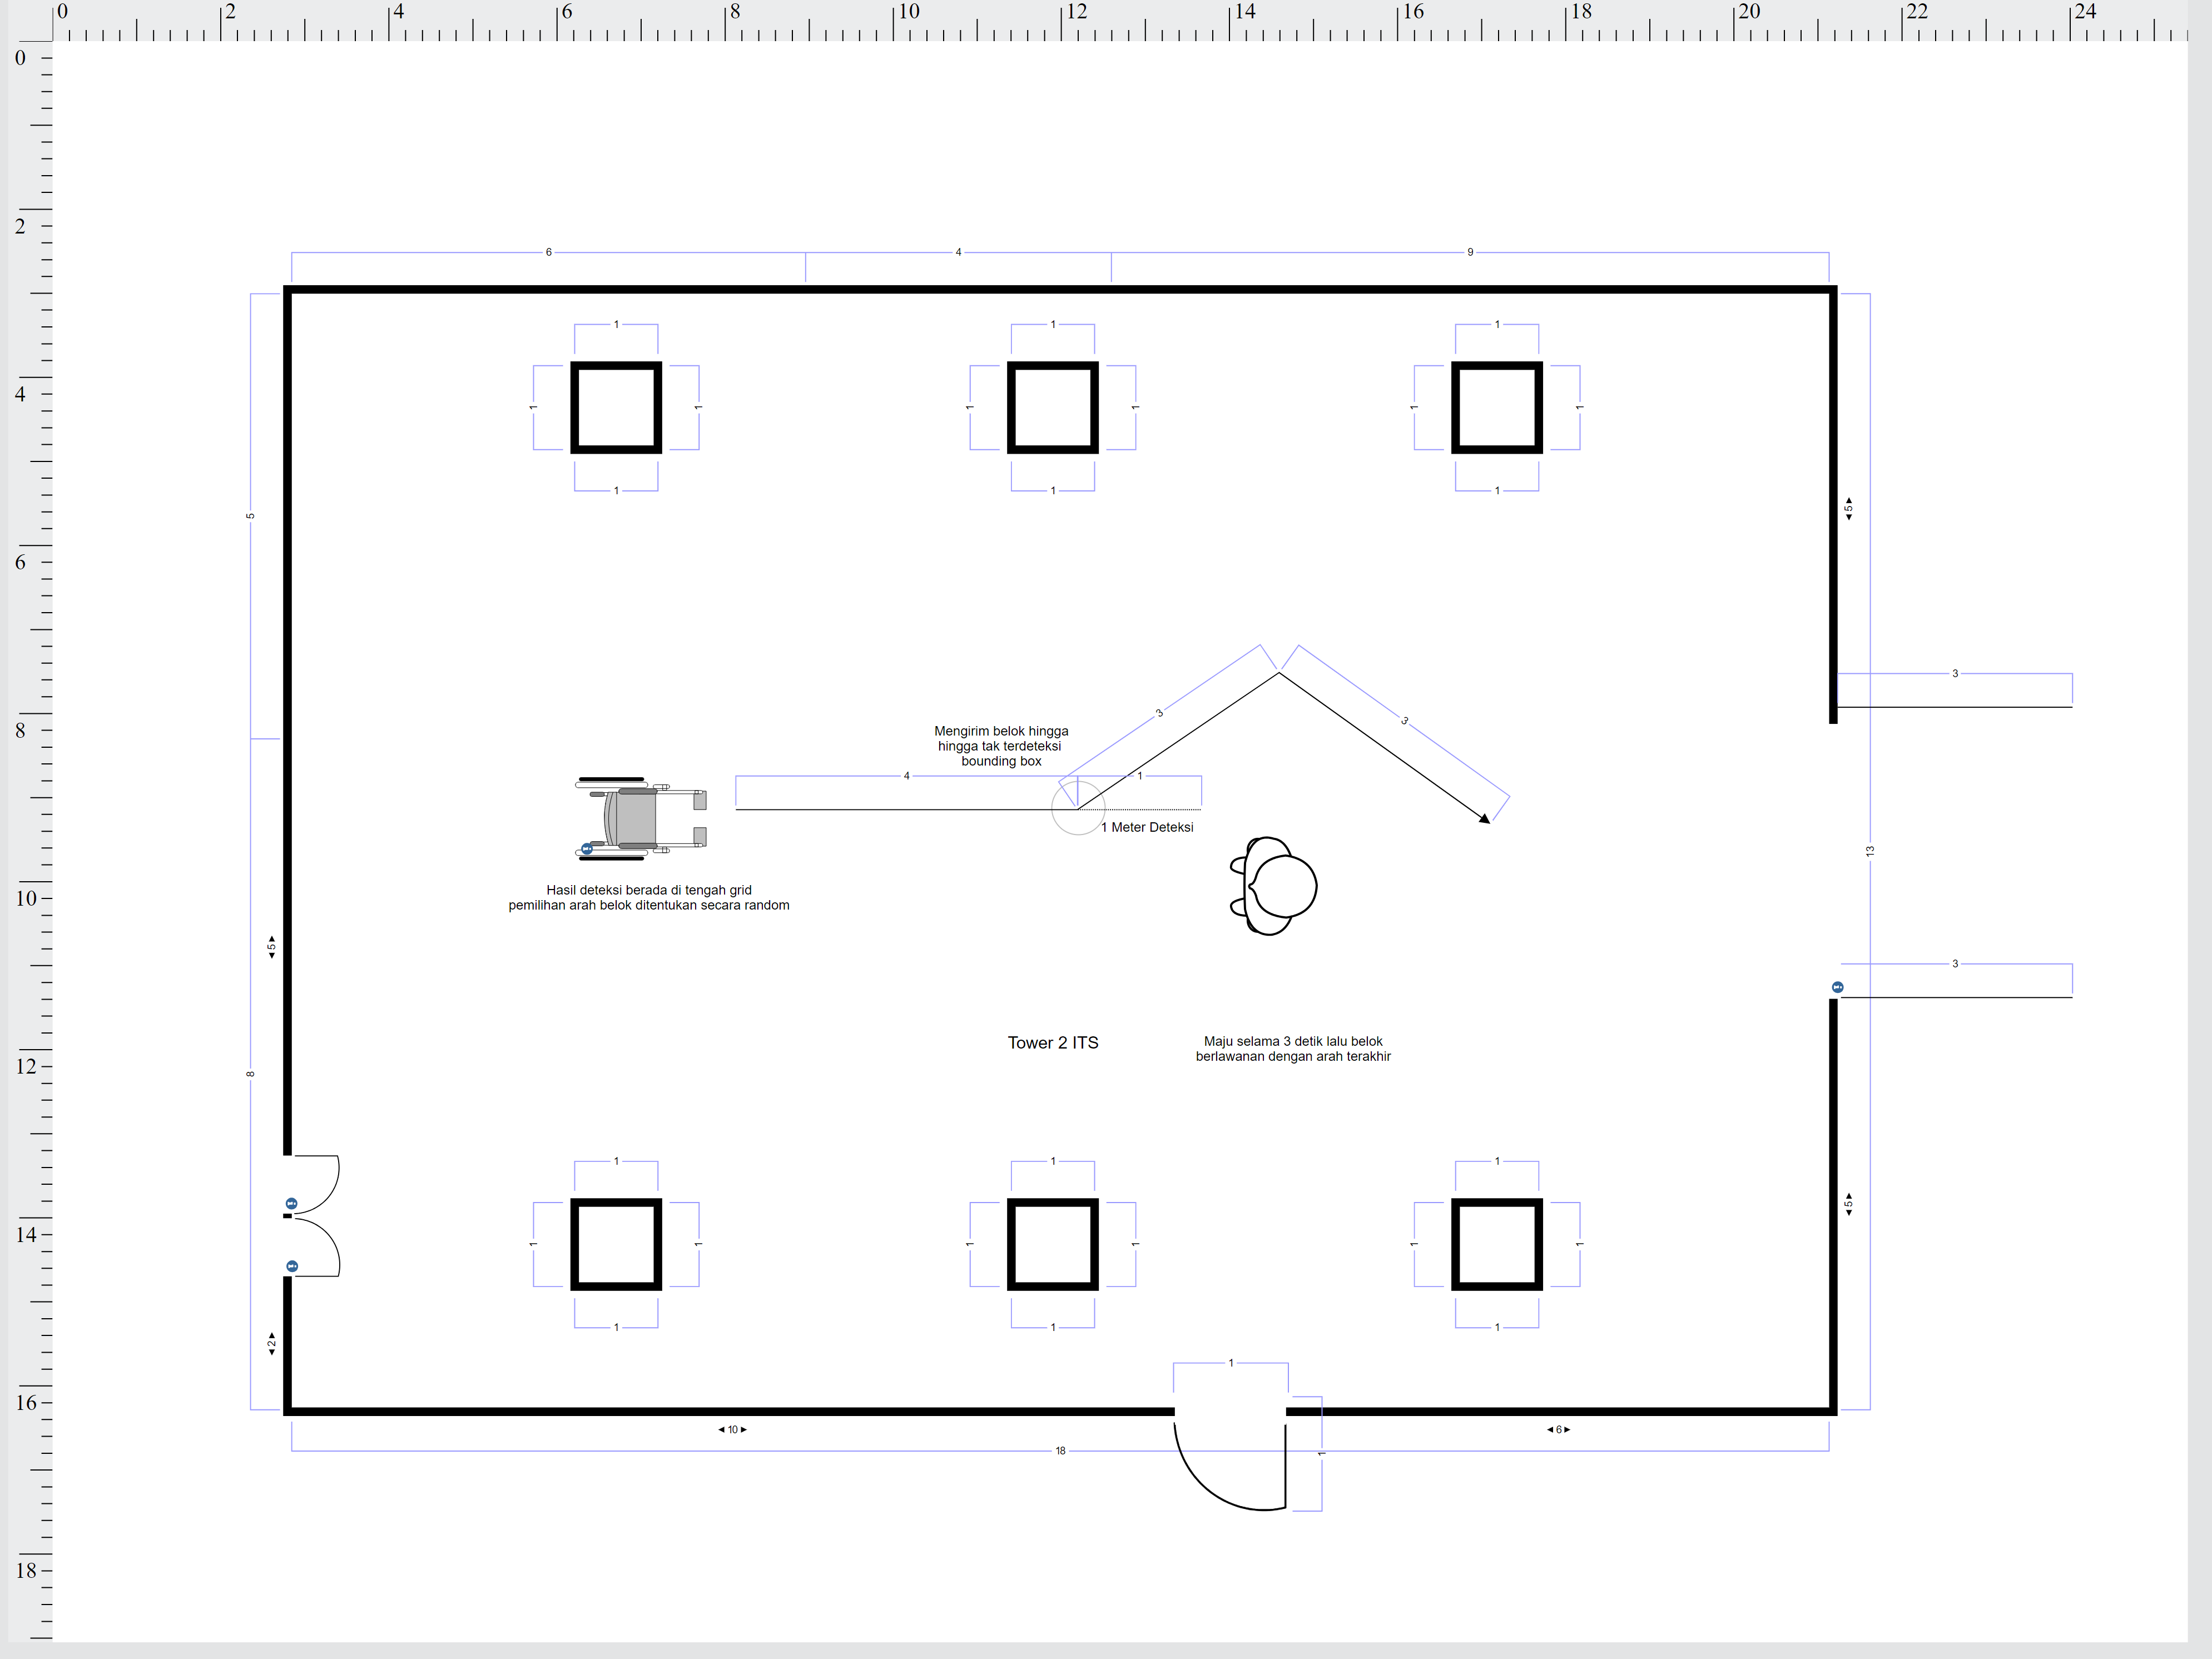
\includegraphics[scale=0.06]{gambar/ManusiaKananNavigasi.png}
  \caption{Avoidance scheme in condition Right Index \textgreater Left}
  \label{fig:Scheme Condition Right Index > Left}
\end{figure}

It can be seen in Figure \ref{fig:Scheme Condition Right Index > Left} that when the wheelchair is 1 meter from detection, it will turn according to the index condition and store this turn direction. If the bounding box is no longer visible, the wheelchair will move forward for 4 seconds, then check the last turn direction. Then the wheelchair will turn again according to the last direction for 5 seconds, then reset the last direction condition. Finally, in this condition, the wheelchair will enter the no detection condition, so it will continue to move forward until the next detection.

\subsubsection{Object detection results on the grid showing a linear position relative to the wheelchair}

In this condition, a command must be added for decision-making where the turn position in this condition, either to the right or left, will not have advantages/disadvantages because in this position the index value is equal on both the right and left. Therefore, a good approach must be made so that this decision-making does not cause errors. In this project, decision-making is based on a random value. Thus, the decision taken can be either to the right or left.

\begin{figure}[H]
    \centering
    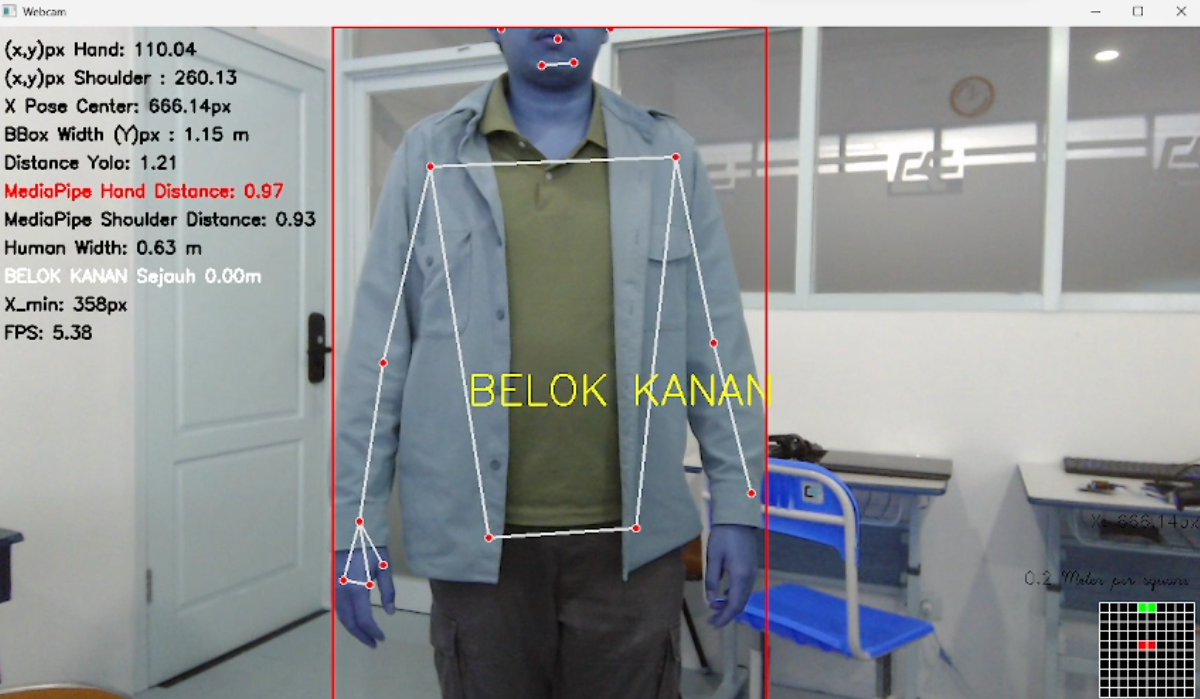
\includegraphics[scale=0.2]{gambar/linierbos.png}
    \caption{Example condition Linear}
    \label{fig:Linear Condition}
\end{figure}

It can be seen in Figure \ref{fig:Linear Condition}, the grid is aligned with the wheelchair position. Thus, the use of random values will be very useful in making decisions when facing such cases.

The wheelchair can only be said to avoid if it returns to its original direction. Thus, Figure \ref{fig:Scheme Condition Linear} is the avoidance scheme that will be followed in this condition.

\begin{figure}[H]
  \centering
  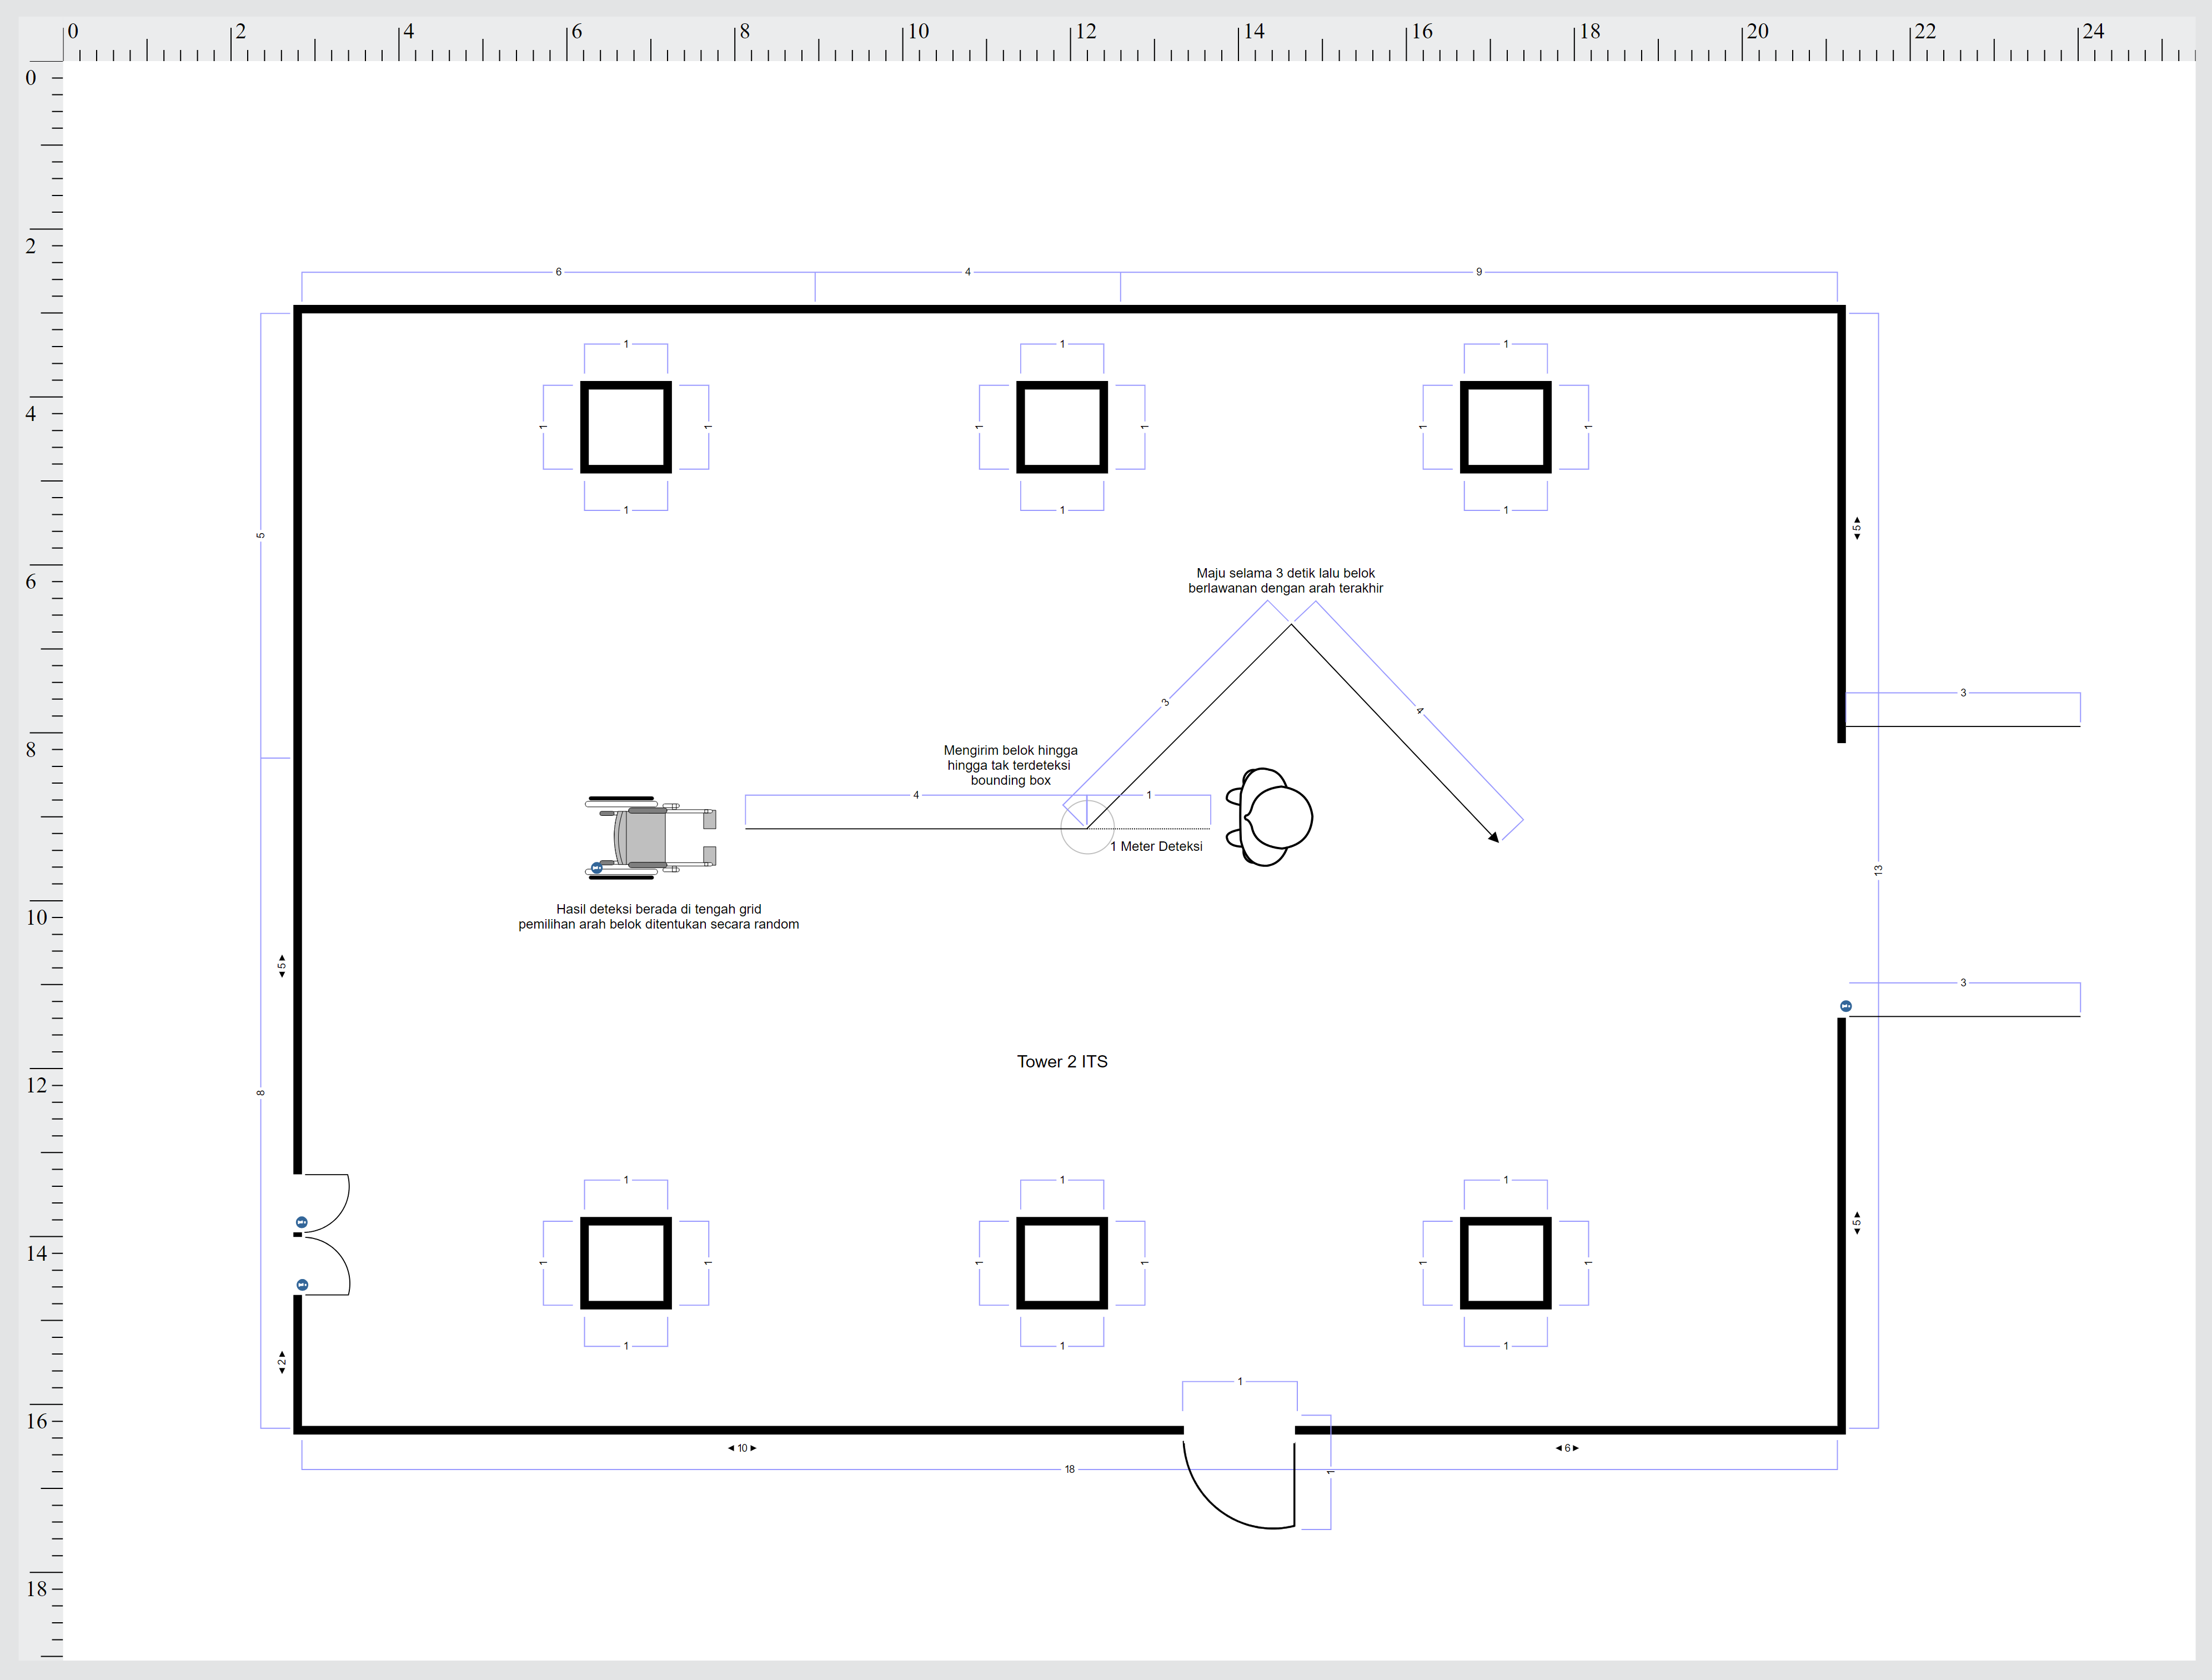
\includegraphics[scale=0.06]{gambar/ManusiaTengahNavigasi.png}
  \caption{Avoidance scheme in condition Linear}
  \label{fig:Scheme Condition Linear}
\end{figure}

It can be seen in Figure \ref{fig:Scheme Condition Linear} that when the wheelchair is 1 meter from detection, it will turn according to the index condition and store this turn direction. If the bounding box is no longer visible, the wheelchair will move forward for 4 seconds, then check the last turn direction. Then the wheelchair will turn again according to the last direction for 5 seconds, then reset the last direction condition. Finally, in this condition, the wheelchair will enter the no detection condition, so it will continue to move forward until the next detection.
